\chapter{预备知识}
\section{基础知识}
\subsection{函数的概念和特性}
\subsubsection{函数}
设$ x $与$ y $是两个变量, $ D $是一个给定的数集, 若对于每一个$ x\in D $, 按照一定的法则$ f $, 有一个唯一确定的$ y $与之对应, 则称$ y $为$ x $的函数, 记为$ y=f(x) $, 称$ x $为自变量, $ y $为因变量, $ D $为定义域.
\subsubsection{反函数}
设函数$ y=f(x) $的定义域为$ D $, 值域为$ R $, 若对于每一个$ y\in R $, 必存在唯一的$ x\in D $使得$ y=f(x) $成立, 则由此定义了一个新的函数$ x=\varphi(y) $, 称这个函数是$ y=f(x) $的反函数, 一般记作$ x=f^{-1}(y) $, 它的定义域为$ R $, 值域为$ D $. \par
\begin{tcolorbox}
\begin{enumerate}
\item 严格单调的函数一定有反函数(严格单调函数不一定是反函数, 如某些分段函数)
\item $ x=f^{-1}(y) $和$ y=f(x) $是同一个函数, 只有写成$ y=f^{-1}(x) $, 图像才关于$ y=x $对称
\end{enumerate}
\end{tcolorbox}
\subsubsection{复合函数}
函数$ u=g(x) $在$ x\in D $上有定义, 函数$ y=f(u) $在$ u\in D_{1} $上有定义, 且$ g(D)\subset D_{1} $, 则称$ y=f(g(x)) $为复合函数, 定义域为$ D $, $ u $为中间变量.
\subsubsection{函数的四种特性和重要结论}
\begin{enumerate}
\item 有界性\par
设$ f(x) $的定义域为$ D $, 数集$ I\subset D $. 若存在某个正数$ M $, 使得对于任一$ x\in I $, 有$ |f(x)|\le M $成立, 则称$ f(x) $在$ I $上有界. 如果这样的$ M $不存在, 则称$ f(x) $在$ I $上无上界.
\item 单调性\par
设$ f(x) $的定义域为$ D $, 区间$ I\subset D $, 如果对于区间上的任一两点$ x_{1},x_{2} $, 当$ x_{1}<x_{2} $的时候有$ f(x_{1})<f(x_{2}) $成立, 则称$ f(x) $在$ I $上单调增加. 反之如果$ f(x_{1})>f(x_{2}) $成立, 则称$ f(x) $在$ I $上单调减少.
\item 奇偶性\par
设$ f(x) $的定义域$ D $关于原点对称. 如果对于任一$ x\in D $, 恒有$ f(x)=f(-x) $, 则称$ f(x) $为偶函数. 如果对于任一$ x\in D $, 恒有$ f(x)=-f(-x) $, 则称$ f(x) $为奇函数. 偶函数的图像关于$ y $轴对称, 奇函数的图像关于原点对称.
\begin{tcolorbox}
\begin{enumerate}
\item 奇函数在$ 0 $点有定义则$ f(0)=0 $
\item 偶函数当$ f'(0) $存在时则$ f'(0)=0 $
\item 函数$ f(x) $和$ -f(x) $关于$ x $轴对称, 函数$ f(x) $和$ f(-x) $关于$ y $轴对称, 函数$ y(x) $和$ -y(-x) $关于原点对称
\item 函数$ f(x) $关于$ x=T $对称$ \Leftrightarrow f(x+T)=f(T-x) $
\end{enumerate}
\end{tcolorbox}
\item 周期性\par
设$ f(x) $的定义域为$ D $, 若存在一个正数$ T $, 使得对于任一$ x\in D $, 有$ x\pm T\in D $, 且$ f(x+T)=f(x) $. 则称$ f(x) $为周期函数, $ T $称为$ f(x) $的周期.
\item 重要结论
\begin{enumerate}
\item 函数和其导函数
\subitem 偶函数的导函数是奇函数
\subitem 奇函数的导函数是偶函数
\subitem 周期函数的周期和其导函数的周期相同
\item 函数和其原函数
\subitem 连续的奇函数的原函数是偶函数
\subitem 连续的偶函数的原函数只有一个是奇函数
\subitem 连续的周期函数和其原函数的周期相同
\item 若$ f(x) $在$ (a,b) $内可导且$ f'(x) $有界, 则$ f(x) $在$ (a,b) $内有界
\end{enumerate}
\end{enumerate}
\subsection{函数的图像}
\subsubsection{直角坐标系}
\begin{enumerate}
\item 常见图像
\begin{enumerate}
\item 基本初等函数与初等函数
\begin{enumerate}
\item 常数函数\par
$ y=C $, $ C $为常数, 图形为平行于$ x $轴的水平直线.
\item 幂函数\par
$ y=x^{\mu} $\ ($ \mu $是实数)
\begin{tcolorbox}
\begin{enumerate}
\item 见到$ \sqrt{u},\sqrt[3]{u} $, 用$ u $来研究最值
\item 见到$ |u| $时, 用$ u^{2} $来研究最值
\item 见到$ u_{1}u_{2}u_{3} $时, 用$ ln(u_{1}u_{2}u_{3})=lnu_{1}+lnu_{2}+lnu_{3} $来研究最值
\item 见到$ \frac{1}{u} $时, 用$ u $来研究最值
\end{enumerate}
\end{tcolorbox}
\item 指数函数
$ y=a^{x} $\ ($ a>0,a\neq 1 $)
\item 对数函数
$ y=log_{a}x $\ ($ a>0,a\neq 1 $)
\begin{tcolorbox}
常用公式: $ x=e^{lnx}\ (x>0), u^{v}=e^{lnu^{v}}=e^{vlnu}\ (u>0) $
\end{tcolorbox}
\item 三角函数
\begin{enumerate}
\item 正弦函数和余弦函数\par
正弦函数$ y=\sin x $, 余弦函数$ y=\cos x $.
\item 正切函数和余切函数\par
正切函数$ y=\tan x $, 余切函数$ y=\cot x $.\par
\begin{figure}[H]
\centering
\begin{subfigure}{.475\linewidth}
\centering
\begin{tikzpicture}[
]
\begin{axis}[
width=\linewidth,
axis lines=middle,
xmin=-4.3,
xmax=4.3,
ymin=-4.5,
ymax=4.5,
xlabel=$ x $,
ylabel=$ y $,
xlabel=$ x $,
xlabel style={below},
ylabel=$ y $,
ylabel style={left},
xtick={-pi/2,pi/2},
xticklabels={$ -\frac{\pi}{2} $,$ \frac{\pi}{2} $},
xticklabel style={left,yshift=-0.5em},
ytick={1},
yticklabels={$ 1 $},
extra y ticks={-1},
extra y tick labels={$ -1 $},
extra y tick style={tick label style={right,yshift=-1em}},
]
\addplot [black,samples=1000]{tan(deg(x))};
\end{axis}
\end{tikzpicture}
\caption{正切函数图像}
\end{subfigure}
\hspace{.1em}
\begin{subfigure}{.475\linewidth}
\centering
\begin{tikzpicture}[
]
\begin{axis}[
width=\linewidth,
axis lines=middle,
xmin=-4.3,
xmax=4.3,
ymin=-4.5,
ymax=4.5,
xlabel=$ x $,
xlabel style={below},
ylabel=$ y $,
ylabel style={left},
xtick={-pi/2,pi/2},
xticklabels={$ -\frac{\pi}{2} $,$ \frac{\pi}{2} $},
xticklabel style={left,yshift=-0.5em},
ytick={1},
yticklabels={$ 1 $},
extra y ticks={-1},
extra y tick labels={$ -1 $},
extra y tick style={tick label style={right,yshift=-1em}},
]
\addplot [black,samples=1000]{1/tan(deg(x))};
\end{axis}
\end{tikzpicture}
\caption{余切函数图像}
\end{subfigure}
\end{figure}
\item 正割函数和余割函数\par
正割函数$ y=\sec x $, 余割函数$ y=\csc x $.
\begin{figure}[H]
\centering
\begin{subfigure}{.475\linewidth}
\centering
\begin{tikzpicture}[
]
\begin{axis}[
width=\linewidth,
axis lines=middle,
xmin=-4.3,
xmax=4.3,
ymin=-4.5,
ymax=4.5,
xlabel=$ x $,
ylabel=$ y $,
xtick={-pi/2,pi/2},
xticklabels={$ -\frac{\pi}{2} $,$ \frac{\pi}{2} $},
xticklabel style={left,yshift=-0.5em},
ytick={-1,1},
yticklabels={$ -1 $,$ 1 $},
yticklabel style={below,xshift=-1em,yshift=0.4em},
]
\addplot [black,samples=1000]{1/cos(deg(x))};
\end{axis}
\end{tikzpicture}
\caption{正割函数图像}
\end{subfigure}
\begin{subfigure}{.475\linewidth}
\begin{tikzpicture}[
]
\begin{axis}[
width=\linewidth,
axis lines=middle,
xmin=-4.3,
xmax=4.3,
ymin=-4.5,
ymax=4.5,
xlabel=$ x $,
ylabel=$ y $,
ylabel style={left},
xtick={pi/2},
xticklabels={$ \frac{\pi}{2} $},
extra x ticks={-pi/2},
extra x tick labels={$ -\frac{\pi}{2} $},
extra x tick style={tick label style={above}},
ytick={1},
yticklabels={$ 1 $},
extra y ticks={-1},
extra y tick labels={$ -1 $},
extra y tick style={tick label style={right,yshift=-0.5em}},
]
\addplot [black,samples=1000]{1/sin(deg(x))};
\end{axis}
\end{tikzpicture}
\caption{余割函数图像}
\end{subfigure}
\end{figure}
\end{enumerate}
\item 反三角函数
\begin{enumerate}
\item 反正弦函数和反余弦函数\par
反正弦函数$ y=\arcsin x $, 反余弦函数$ y=\arccos x $.
\begin{figure}[H]
\centering
\begin{subfigure}{.475\linewidth}
\centering
\begin{tikzpicture}[
]
\begin{axis}[
width=\linewidth,
axis lines=middle,
domain=-1:1,
xmin=-2,
xmax=2,
ymin=-2,
ymax=2,
xlabel=$ x $,
ylabel=$ y $,
xtick={-1,1},
ytick={-pi/2,pi/2},
yticklabels={$ -\frac{\pi}{2} $, $ \frac{\pi}{2} $},
]
\addplot [black,samples=1000]{asin(x)/180*pi};
\end{axis}
\end{tikzpicture}
\caption{反正弦函数图像}
\end{subfigure}
\begin{subfigure}{.475\linewidth}
\begin{tikzpicture}[
]
\begin{axis}[
width=\linewidth,
axis lines=middle,
domain=-1:1,
xmin=-2,
xmax=2,
ymin=-0.5,
ymax=4,
xlabel=$ x $,
ylabel=$ y $,
ytick={pi/2,pi},
yticklabels={$ \frac{\pi}{2} $, $ \pi $},
xtick={-1,1},
xticklabels={$ -1 $,$ 1 $},
]
\addplot [black,samples=1000]{acos(x)/180*pi};
\end{axis}
\end{tikzpicture}
\caption{反余弦函数图像}
\end{subfigure}
\end{figure}
\item 反正切函数和反余切函数\par
反正切函数$ y=\arctan x $, 反余切函数$ y=\arccot x $
\begin{figure}[H]
\centering
\begin{subfigure}{.475\linewidth}
\centering
\begin{tikzpicture}[
]
\begin{axis}[
width=\linewidth,
axis lines=middle,
xmin=-2,
xmax=2,
ymin=-2,
ymax=2,
xlabel=$ x $,
ylabel=$ y $,
xtick={\empty},
ytick={-pi/2,pi/2},
yticklabels={$ -\frac{\pi}{2} $, $ \frac{\pi}{2} $},
]
\addplot [black,samples=1000]{atan(x)/180*pi};
\end{axis}
\end{tikzpicture}
\caption{反正切函数图像}
\end{subfigure}
\begin{subfigure}{.475\linewidth}
\begin{tikzpicture}[
]
\begin{axis}[
width=\linewidth,
axis lines=middle,
xmin=-2,
xmax=2,
ymin=-0.5,
ymax=4,
xlabel=$ x $,
ylabel=$ y $,
ytick={pi/2,pi},
yticklabels={$ \frac{\pi}{2} $, $ \pi $},
xtick={\empty},
]
\addplot [black,samples=1000]{(pi/2)-(atan(x))/180*pi};
\end{axis}
\end{tikzpicture}
\caption{反余切函数图像}
\end{subfigure}
\end{figure}
\end{enumerate}
\item 初等函数\par
由基本初等函数经过有限次的四则运算, 以及有限次的复合所构成的可以用一个式子表示的函数称为初等函数.
\end{enumerate}
\item 分段函数\par
在自变量的不同范围中, 对应法则不同式子来表示的函数称为分段函数. 一般来说它不是初等函数.
\begin{enumerate}
\item 绝对值函数\par
\begin{equation*}
y=|x|=
\scaleleftright[6pt]{\biggl\{}{
\begin{aligned}
& x,\ x\ge 0 \\
& -x,\ x<0
\end{aligned}
}{.}
\end{equation*}
\item 符号函数\par
\begin{equation*}
y=\text{sgn}\ x=
\scaleleftright[6pt]{\biggl\{}{
\begin{aligned}
& 1,\ x>0 \\
& 0,\ x=0 \\
& -1,\ x<0
\end{aligned}
}{.}
\end{equation*}
\item 取整函数\par
$ y=[x] $, 设$ x $为任一实数, 不超过$ x $的最大整数称为$ x $的整数部分, 记作$ [x] $.
\end{enumerate}
\end{enumerate}
\item 图像变换
\begin{enumerate}
\item 平移变换
\begin{enumerate}
\item 将函数$ y=f(x) $沿$ x $轴向左平移$ x_{0}\ (x_{0}>0) $个单位长度, 得到函数$ f(x+x_{0}) $的图像; 将函数$ y=f(x) $沿$ x $轴向右平移$ x_{0}\ (x_{0}>0) $个单位长度, 得到函数$ f(x-x_{0}) $的图像
\item 将函数$ y=f(x) $沿$ y $轴向上平移$ y_{0}\ (y_{0}>0) $个单位长度, 得到函数$ f(x)+y_{0} $的图像; 将函数$ y=f(x) $沿$ y $轴向下平移$ y_{0}\ (y_{0}>0) $个单位长度, 得到函数$ f(x)-y_{0} $的图像
\end{enumerate}
\item 对称变换
\begin{enumerate}
\item 将函数$ y=f(x) $的图像关于$ x $轴对称, 得到函数$ y=-f(x) $的图像
\item 将函数$ y=f(x) $的图像关于$ y $轴对称, 得到函数$ y=f(-x) $的图像
\item 将函数$ y=f(x) $的图像关于原点对称, 得到函数$ y=-f(-x) $的图像
\item 将函数$ y=f(x) $的图像关于直线$ y=x $对称, 得到函数$ y=f^{-1}(x) $的图像
\item 保留函数$ y=f(x) $在$ x $轴及$ x $轴上方的部分, 把$ x $轴下方的部分关于$ x $轴对称到$ x $轴上方并去掉原来下方的部分, 得到函数$ y=|f(x)| $的图像
\item 保留函数$ y=f(x) $在$ y $轴及$ y $轴右侧的部分, 去掉$ y $轴左侧的部分, 再将$ y $轴右侧图像对称到$ y $轴左侧, 得到函数$ y=f(|x|) $的图像
\end{enumerate}
\item 伸缩变换
\begin{enumerate}
\item 水平伸缩: $ y=f(kx)(k>1) $的图像, 可由$ y=f(x) $的图像上每点的横坐标缩短到原来的$ \frac{1}{k} $倍且纵坐标不变得到. $ y=f(kx)(0<k<1) $的图像, 可由$ y=f(x) $的图像上每点的横坐标伸长到原来的$ \frac{1}{k} $倍且纵坐标不变得到
\item 垂直伸缩: $ y=kf(x)(k>1) $的图像, 可由$ y=f(x) $的图像上每点的纵坐标伸长到原来的$ k $倍且横坐标不变得到; $ y=kf(x)(0<k<1) $的图像, 可由$ y=f(x) $的图像上每点的纵坐标缩短到原来的$ k $倍且横坐标不变得到
\end{enumerate}
\end{enumerate}
\end{enumerate}
\subsubsection{极坐标系}
\begin{enumerate}
\item 用描点法画常见图像\par
\begin{enumerate}
\item 心形线\par
$ r=a(1-\cos \theta)(a>0) $
\begin{figure}[H]
\centering
\begin{tikzpicture}[
>=stealth,
]
\draw[->] (0,0)node[left]{$ 0 $} to (1,0)node[right]{$ x $};
\draw[domain=0:360,samples=1000,scale=.7] plot (\x:{2*(1-cos(\x))});
\end{tikzpicture}
\caption{心形线}
\end{figure}
\item 玫瑰线\par
$ r=a\sin 3\theta (a>0) $
\begin{figure}[H]
\centering
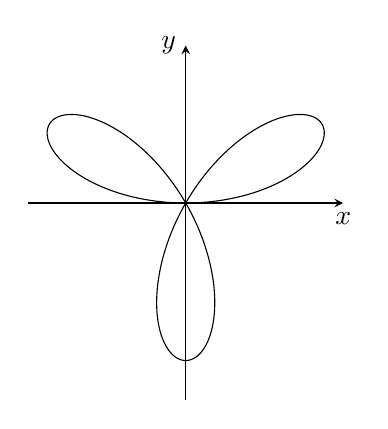
\begin{tikzpicture}[
>=stealth,
]
\draw[->] (-2,0) to (2,0)node[below]{$ x $};
\draw[->] (0,-2.5) to (0,2)node[left]{$ y $};
\draw[domain=0:360,samples=1000,scale=1] plot (\x:{2*sin(3*\x)});
\end{tikzpicture}
\caption{玫瑰线}
\end{figure}
\item 阿基米德螺线\par
$ r=a\theta (a>0,\theta \ge 0) $
\begin{figure}[H]
\centering
\begin{tikzpicture}[
>=stealth,
]
\draw[->] (0,0)node[left]{$ 0 $} to (3,0)node[below]{$ x $};
\draw[domain=0:360,samples=1000,scale=.2] plot (\x:{2*(\x/180*pi)});
\end{tikzpicture}
\caption{阿基米德螺线}
\end{figure}
\item 伯努利双纽线\par
$ r^{2}=a^{2}\cos 2\theta(a>0) $或$ r^{2}=a^{2}\sin 2\theta(a>0) $.
\begin{figure}[H]
\centering
\begin{subfigure}{.475\linewidth}
\centering
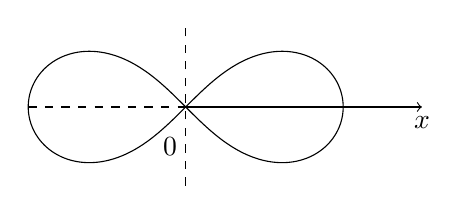
\begin{tikzpicture}
\draw[->] (0,0) to (3,0)node[below]{$ x $};
\node at (-.2,-.5){$ 0 $};
\draw[dashed] (0,-1) to (0,1);
\draw[dashed] (-2,0) to (0,0);
\draw[domain=0:45,samples=1000] plot (\x:{sqrt(4*cos(2*\x))});
\draw[domain=135:225,samples=1000] plot (\x:{sqrt(4*cos(2*\x))});
\draw[domain=315:360,samples=1000] plot (\x:{sqrt(4*cos(2*\x))});
\end{tikzpicture}
\caption{$ r^{2}=a^{2}\cos 2\theta $}
\end{subfigure}
\hfill
\begin{subfigure}{.475\linewidth}
\centering
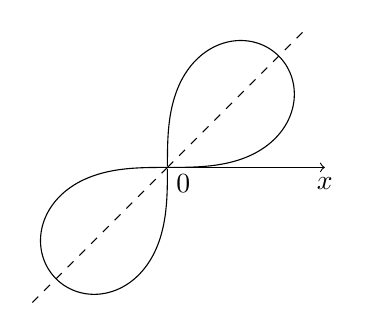
\begin{tikzpicture}
\draw[->] (0,0) to (2,0)node[below]{$ x $};
\node at (.2,-.2){$ 0 $};
\draw[domain=0:90,samples=1000,] plot (\x:{sqrt(4*sin(2*\x))});
\draw[domain=180:270,samples=1000,] plot (\x:{sqrt(4*sin(2*\x))});
\draw[dashed] (0,0) to (45:2.5);
\draw[dashed] (0,0) to (225:2.5);
\end{tikzpicture}
\caption{$ r^{2}=a^{2}\sin 2\theta $}
\end{subfigure}
\caption{伯努利双纽线}
\end{figure}
\end{enumerate}
\end{enumerate}
\subsubsection{参数方程}
\begin{enumerate}
\item 摆线\par
\begin{equation*}
\scaleleftright[6pt]{\biggl\{}{
\begin{aligned}
& x=r(t-\sin t) \\
& y=r(1-\cos t)
\end{aligned}
}{.}
\end{equation*}
\begin{figure}[H]
\centering
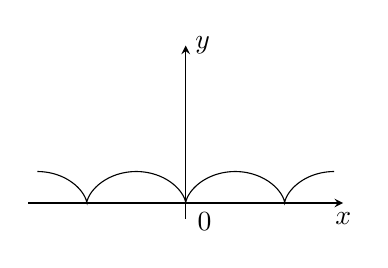
\begin{tikzpicture}[
>=stealth,
scale=2,
]
\draw[->] (-1,0) to (1,0)node[below]{$ x $};
\draw[->] (0,-.1) to (0,1)node[right]{$ y $};
\node at (.12,-.12){$ 0 $};
\draw[domain=-540:540][samples=1000] plot({(\x/180*pi-sin(\x))*0.1},{(1-cos(\x))*0.1});
\end{tikzpicture}
\caption{摆线}
\end{figure}
\item 星形线\par
\begin{equation*}
\scaleleftright[6pt]{\biggl\{}{
\begin{aligned}
& x=r\cos^{3}t \\
& y=r\sin^{3}t
\end{aligned}
}{.}
\end{equation*}
\begin{figure}[H]
\centering
\begin{tikzpicture}[
>=stealth,
scale=2,
]
\draw[->] (-1,0) to (1.2,0)node[below]{$ x $};
\draw[->] (0,-1) to (0,1.2)node[right]{$ y $};
\node at (.12,-.12){$ 0 $};
\draw[domain=0:360][samples=1000] plot({(cos(\x))^3},{(sin(\x))^3});
\end{tikzpicture}
\caption{星形线}
\end{figure}
\end{enumerate}
\subsection{常用基础知识}
\subsubsection{数列}
\begin{enumerate}
\item 等差数列\par
首项为$ a_{1} $,公差为$ d(d\neq 0) $的数列$ a_{1},a_{1}+d,a_{1}+2d,...,a_{1}+(n-1)d,... $.
\begin{enumerate}
\item 通项公式: $ a_{n}=a_{1}+(n-1)d $
\item 前$ n $项的和: $ S_{n}=\frac{n}{2}(a_{1}+a_{n})=\frac{n}{2}[2a_{1}+(n-1)d] $
\end{enumerate}
\item 等比数列\par
首项为$ a_{1} $, 公比为$ r(r\neq 0) $的数列$ a_{1},a_{1}r,...,a_{1}r^{n-1},... $.
\begin{enumerate}
\item 通项公式: $ a_{n}=a_{1}r^{n-1} $
\item 前$ n $项的和$ S_{n}=\scaleleftright[6pt]{\biggl\{}{\begin{aligned}
& na_{1}\ & r=1 \\
& \frac{a_{1}(1-r^{n})}{1-r} & r\neq 1
\end{aligned}}{.} $
\item 一些常见数列前$ n $项的和\par
\begin{enumerate}
\item $ \sum_{k=1}^{n}k=1+2+3+...+n=\frac{n(1+n)}{2} $
\item $ \sum_{k=1}^{n}k^{2}=1^{2}+2^{2}+...+n^{2}=\frac{n(n+1)(2n+1)}{6} $
\item $ \sum_{k=1}^{n}\frac{1}{k(k+1)}=\frac{1}{1\times 2}+\frac{1}{2\times 3}+...+\frac{1}{n(n+1)}=\frac{n}{n+1} $
\end{enumerate}
\end{enumerate}
\end{enumerate}
\subsubsection{三角函数}
\begin{enumerate}
\item 三角函数的基本关系
\[ \begin{split}&\csc \alpha=\frac{1}{\sin \alpha},\ \sec \alpha=\frac{1}{\cos \alpha},\ \cot \alpha=\frac{1}{\tan \alpha}\\& \sin^{2}\alpha +\cos^{2}\alpha =1,\ 1+\tan^{2}\alpha = \sec^{2}\alpha,\ 1+\cot^{2}\alpha =\csc^{2}\alpha\\ &\tan \alpha=\frac{\sin \alpha}{\cos \alpha},\ \cot \alpha=\frac{\cos \alpha}{\sin \alpha}\end{split}\]
\item 重要公式
\item 倍角公式
\[ \begin{split}
& \sin 2\alpha=2\sin \alpha \cos \alpha,\ \cos 2\alpha =\cos^{2}\alpha -\sin^{2}\alpha =1-2\sin^{2}\alpha\\&=2\cos^{2}\alpha -1,\ \tan 2\alpha =\frac{2\tan \alpha}{1-\tan^{2}\alpha}
\end{split} \]
\item 半角公式
\[ \begin{split}
& \sin^{2}\frac{\alpha}{2}=\frac{1}{2}(1-\cos \alpha),\ \cos^{2}\frac{\alpha}{2}=\frac{1}{2}(1+\cos \alpha) \\
& \tan \frac{\alpha}{2}=\frac{1-\cos \alpha}{\sin \alpha}=\frac{\sin \alpha}{1+\cos \alpha}=\pm \sqrt{\frac{1-\cos \alpha}{1+\cos \alpha}}
\end{split} \]
\item 和差公式
\[ \begin{split}
& \sin(\alpha \pm \beta)=\sin\alpha\cos\beta \pm \cos\alpha\sin\beta \\
& \cos(\alpha \pm \beta)=\cos\alpha\cos\beta \mp \sin\alpha\sin\beta \\
& \tan(\alpha \pm \beta)=\frac{\tan\alpha \pm \tan\beta}{1 \mp \tan\alpha\tan\beta}
\end{split} \]
\item 积化和差公式
\[ \begin{split}
& \sin\alpha\cos\beta = \frac{1}{2}[\sin(\alpha + \beta) + \sin(\alpha - \beta)] \\
& \cos\alpha\sin\beta = \frac{1}{2}[\sin(\alpha + \beta) - \sin(\alpha - \beta)] \\
& \cos\alpha\cos\beta = \frac{1}{2}[\cos(\alpha + \beta) + \cos(\alpha - \beta)] \\
& \sin\alpha\sin\beta = -\frac{1}{2}[\cos(\alpha + \beta) - \cos(\alpha - \beta)] \\
\end{split} \]
\item 和差化积公式
\[ \begin{split}
& \sin\alpha + \sin\beta = 2\sin\frac{\alpha+\beta}{2}\cos\frac{\alpha - \beta}{2} \\
& \sin\alpha - \sin\beta = 2\cos\frac{\alpha+\beta}{2}\sin\frac{\alpha - \beta}{2} \\
& \cos\alpha + \cos\beta = 2\cos\frac{\alpha+\beta}{2}\cos\frac{\alpha - \beta}{2} \\
& \cos\alpha - \cos\beta = -2\sin\frac{\alpha+\beta}{2}\sin\frac{\alpha - \beta}{2} \\
\end{split} \]
\item 万能公式\par
若$ u=\tan \frac{x}{2}(-\pi<x<\pi) $, 则$ \sin x=\frac{2u}{1+u^{2}} $, $ \cos x=\frac{1-u^{2}}{1+u^{2}} $.
\end{enumerate}
\subsubsection{指数运算法则}
\vspace*{-2em}
\[ \begin{split}
& a^{\alpha}\cdot a^{\beta}=a^{\alpha + \beta},\  \frac{a^{\alpha}}{a^{\beta}}=a^{\alpha-\beta} \\
& (a^{\alpha})^{\beta}=a^{\alpha \beta},\ (ab)^{\alpha}=a^{\alpha}b^{\alpha},\ (\frac{a}{b})^{\alpha}=\frac{a^{\alpha}}{b^{\alpha}}
\end{split} \]
\subsubsection{对数运算法则}
\begin{enumerate}
\item $ \log_{a}(MN)=\log_{a}M+\log_{a}N  $
\item $ \log_{a}\frac{M}{N}=\log_{a}M-\log_{a}N $
\item $ \log_{a}^{n}=n\log_{a}M $
\item $ \log_{a}\sqrt[n]{M}=\frac{1}{n}\log_{a}M $
\end{enumerate}
\subsubsection{一元二次方程基础}
\begin{enumerate}
\item 一元二次方程: $ ax^{2}+bx+c=0(a\neq 0) $
\item 根的公式: $ x_{1,2}=\frac{-b\pm \sqrt{b^{2}-4ac}}{2a} $
\item 根和系数的关系: $ x_{1}+x_{2}=-\frac{b}{a},\ x_{1}x_{2}=\frac{c}{a} $
\item 判别式: $ \Delta=b^{2}-4ac $
\item 抛物线定点坐标: $ (-\frac{b}{2a},c-\frac{b^{2}}{4a}) $
\end{enumerate}
\subsubsection{因式分解公式}
\begin{enumerate}
\item $ (a+b)^{2}=a^{2}+b^{2}+2ab $
\item $ (a-b)^{2}=a^{2}+b^{2}-2ab $
\item $ (a+b)^{3}=a^{3}+3a^{2}b+3b^{2}a+b^{3} $
\item $ (a-b)^{3}=a^{3}-3a^{2}b+3b^{2}a-b^{3} $
\item $ a^{3}+b^{3}=(a+b)(a^{2}-ab+b^{2}) $
\item $ a^{3}-b^{3}=(a-b)(a^{2}+ab+b^{2}) $
\item $ a^{2}-b^{2}=(a+b)(a-b) $
\item 二项式定理: $ (a+b)^{n}=\sum_{k=0}^{n}C_{n}^{k}a^{n-k}b^{k} $
\end{enumerate}
\subsubsection{阶乘和双阶乘}
\begin{enumerate}
\item $ n!=1\cdot 2\cdot 3\cdot ... \cdot n $, 规定$ 0!=1 $
\item $ (2n)!!=2\cdot 4\cdot 6\cdot ... \cdot (2n)=2^{n}n! $
\item $ 2(n-1)!!=1\cdot 3\cdot 5\cdot ... \cdot (2n-1) $
\end{enumerate}
\subsubsection{常用不等式}
\begin{enumerate}
\item 设$ a,b $为实数, 则有:
\begin{enumerate}
\item $ |a\pm b|\le |a|+|b| $
\item $ ||a|-|b||\le |a-b| $
\end{enumerate}
\item $ \sqrt{ab}\le \frac{a+b}{2}\le \sqrt{\frac{a^{2}+b^{2}}{2}}(a,b>0) $
\item 设$ a>b>0 $, 则$ \scaleleftright[6pt]{\biggl\{}{\begin{aligned}
& \text{当}n>0\text{时}, a^{n}>b^{n} \\
& \text{当}n<0\text{时}, a^{n}<b^{n}
\end{aligned}}{.} $
\item 若$ 0<a<x<b,0<c<y<d $, 则$ \frac{c}{b}<\frac{y}{x}<\frac{d}{a} $
\item $ \sin x<x<\tan x(0<x<\frac{\pi}{2}) $
\item $ \sin x<x(x>0) $
\item $ \arctan x\le x\le \arcsin x(0\le x\le 1)$
\item $ e^{x}\ge x+1(\forall x) $
\item $ x-1\ge \ln x(x>0) $
\item $ \frac{1}{1+x}<\ln (1+\frac{1}{x})<\frac{1}{x}(x>0) $
\end{enumerate}
\chapter{数列极限}
\section{基础知识}
\subsection{数列极限的定义}
设$ \{x_{n}\} $为一数列, 若存在常数$ a $, 对于任意的$ \epsilon >0 $, 总存在正整数$ N $, 使得当$ n>N $的时候, $ |x_{n}-a|<\epsilon $恒成立, 则称数$ a $是数列$ \{x_{n}\} $的极限, 或者称数列$ \{x_{n}\} $收敛于$ a $, 记为
\begin{equation*}
\lim_{n\rightarrow \infty} x_{n} = a\ or\ x_{n}\rightarrow a(n\rightarrow \infty).
\end{equation*}
\subsection{收敛数列的性质}
\begin{enumerate}
\item 唯一性: 若数列存在极限, 则极限唯一
\item 有界性: 若数列存在极限, 则数列有界
\item 保号性
\begin{enumerate}
\item 脱帽: 设有数列$ \{x_{n}\} $, 若$ \lim\limits_{n\rightarrow \infty}x_{n}=a>0(\text{或}<0)\Rightarrow $ 存在正整数$ N $, 当$ n>N $时, 有$ x_{n}>0(\text{或}x_{n}<0) $
\item 戴帽: 设有数列$ \{x_{n}\} $, 若存在正整数$ N $, 当$ n>N $时, 有$ x_{n}\ge 0 $, 且数列存在极限$ \Rightarrow \lim\limits_{n\rightarrow \infty}x_{n}=a\ge 0 $
\end{enumerate}
\end{enumerate}
\subsection{极限运算规则}
设$ \lim\limits_{n\rightarrow \infty}x_{n}=a, \lim\limits_{n\rightarrow \infty}y_{n}=b $, 则
\begin{enumerate}
\item $ \lim\limits_{n\rightarrow \infty}(x_{n}\pm y_{n})=a\pm b $
\item $ \lim\limits_{n\rightarrow \infty}x_{n}y_{n}=ab $
\item 若$ b\neq 0, y_{n}\neq 0 \Rightarrow \lim\limits_{n\rightarrow \infty}\frac{x_{n}}{y_{n}}=\frac{a}{b}$
\end{enumerate}
\subsection{夹逼准则}
若数列$ \{x_{n}\}, \{y_{n}\} $及$ \{z_{n}\} $满足条件:
\begin{enumerate}
\item $ y_{n}\le x_{n}\le z_{n}(n=1,2,3...) $
\item $ \lim\limits_{n\rightarrow \infty}y_{n}=a, \lim\limits_{n\rightarrow \infty}z_{n}=a $
\end{enumerate}\par
则数列$ \{x_{n}\} $的极限存在, 且$ \lim\limits_{n\rightarrow \infty}x_{n}=a $.
\subsection{单调有界准则}
单调有界数列必有极限.
\section{习题}
\chapter{函数极限}
\section{基础知识}
\subsection{邻域}
\subsubsection{一维}
\begin{enumerate}
\item 邻域: 点$ x_{0} $的邻域为数轴上以$ x_{0} $为中心的任何开区间, 记作$ U(x_{0}) $
\item $ \delta $邻域: 点$ x_{0} $的$ \delta $邻域为$ (x_{0}-\delta,x_{0}+\delta) $, 记作$ U(x_{0},\delta) $
\item 去心$ \delta $邻域: 点$ x_{0} $的去心$ \delta $邻域为$ (x_{0}-\delta,x_{0})\cup (x_{0},x_{0}+\delta) $, 记作$ \mathring{U}(x_{0},\delta) $
\item 左右$ \delta $邻域
\begin{enumerate}
\item 左邻域: 点$ x_{0} $的左邻域为$ (x_{0}-\delta,x_{0}) $, 记作$ U^{+}(x_{0},\delta) $
\item 右邻域: 点$ x_{0} $的右邻域为$ (x_{0},x_{0}+\delta) $, 记作$ U^{-}(x_{0},\delta) $
\end{enumerate}
\end{enumerate}
\subsubsection{二维}
\begin{enumerate}
\item $ \delta $邻域: 与点$ P_{0}(x_{0},y_{0}) $的距离小于$ \delta $的点$ P(x,y) $的全体, 称为点$ P_{0} $的$ \delta $邻域, 记作$ U(P_{0},\delta) $
\item 去心$ \delta $邻域: 与点$ P_{0}(x_{0},y_{0}) $的距离小于$ \delta $但不等于0的点$ P(x,y) $的全体, 称为点$ P_{0} $的去心$ \delta $邻域, 记作$ \mathring{U}(P_{0},\delta) $
\end{enumerate}
\subsection{函数极限的定义}
设函数$ f(x) $在某点$ x_{0} $的某一去心邻域内有定义. 若存在常数$ A $, 对于任意给定的$ \epsilon >0 $, 总存在正数$ \delta $, 使得当$ 0<|x-x_{0}|<\delta $时, 满足$ |f(x)-A|<\epsilon $, 则$ A $就叫作函数$ f(x) $当$ x\rightarrow x_{0} $时的极限, 记为
\begin{equation*}
\lim\limits_{x\rightarrow \infty} f(x)=A\ or \ f(x)\rightarrow A\ (x\rightarrow x_{0})
\end{equation*}\par
用$ \epsilon -X $语言表示为: $ \lim\limits_{x\rightarrow \infty}f(x)=A\Leftrightarrow \forall \epsilon >0, \exists X>0 $, 当$ |x|>X $时, 有$ |f(x)-A|<\epsilon $
\subsubsection{单侧极限}
\begin{enumerate}
\item 左极限: $ \lim\limits_{x\rightarrow x_{0}^{-}}f(x)=A\ or\ f(x_{0}^{-})=A $
\item 右极限: $ \lim\limits_{x\rightarrow x_{0}^{+}}f(x)=A\ or\ f(x_{0}^{+})=A $
\end{enumerate}
\subsubsection{充要条件}
函数$ f(x) $在点$ x_{0} $处有极限的充要条件分别有:
\begin{enumerate}
\item $ \lim\limits_{x\rightarrow x_{0}}f(x)=A\Leftrightarrow \lim\limits_{x\rightarrow x_{0}^{-}}f(x)=\lim\limits_{x\rightarrow x_{0}^{+}}f(x)=A $
\item $ \lim\limits_{x\rightarrow x_{0}}f(x)=A\Leftrightarrow f(x)=A+\alpha(x), \lim\limits_{x\rightarrow x_{0}}\alpha(x)=0 $
\end{enumerate}
\subsection{函数极限的性质}
\begin{enumerate}
\item 唯一性: 若函数存在极限, 则极限唯一
\item 局部有界性: 若函数存在极限, 则函数在某一区间内有界
\item 局部保号性
\begin{enumerate}
\item 脱帽: 设有函数$ f(x) $, 若$ \lim\limits_{x\rightarrow x_{0}}f(x)=A>0(\text{或}A<0) \Rightarrow $ 存在常数$ \delta $, 当$ 0<|x-x_{0}|<\delta $时, 有$ f(x)>0(\text{或}f(x)<0) $
\item 戴帽: 设有函数$ f(x) $, 若存在常数$ \delta $, 当$ 0<|x-x_{0}|<\delta $时, 有$ f(x)\ge 0(\text{或}f(x)\le 0) \Rightarrow \lim\limits_{x\rightarrow x_{0}}f(x)=A\ge 0(\text{或}\le 0) $
\end{enumerate}
\end{enumerate}
\subsection{极限运算法则}
设$ \lim\limits_{x\rightarrow x_{0}}f(x)=A, \lim\limits_{x\rightarrow x_{0}}g(x)=B $, 则
\begin{enumerate}
\item $ \lim\limits_{x\rightarrow x_{0}}[kf(x)\pm lg(x)]=k \lim\limits_{x\rightarrow x_{0}}f(x)\pm l \lim\limits_{x\rightarrow x_{0}}g(x)=kA\pm lB $, 其中$ k,l $为常数
\item $ \lim\limits_{x\rightarrow x_{0}}[f(x)\cdot g(x)]=\lim\limits_{x\rightarrow x_{0}}f(x)\cdot \lim\limits_{x\rightarrow x_{0}}g(x)=A\cdot B $
\item $ \lim\limits_{x\rightarrow x_{0}}\frac{f(x)}{g(x)}=\frac{\lim\limits_{x\rightarrow x_{0}}f(x)}{\lim\limits_{x\rightarrow x_{0}}g(x)}=\frac{A}{B}(B\neq 0) $
\item $ \lim\limits_{x\rightarrow x_{0}}[f(x)]^{n}=[\lim\limits_{x\rightarrow x_{0}}f(x)]^{n} $, $ n $为正整数
\end{enumerate}
\subsection{夹逼准则}
若函数$ f(x), g(x) $及$ h(x) $满足条件:
\begin{enumerate}
\item $ g(x)\le f(x)\le h(x) $
\item $ \lim\limits_{x\rightarrow x_{0}}g(x)=A, \lim\limits_{x\rightarrow x_{0}}h(x)=A $
\end{enumerate}\par
则函数$ f(x) $极限存在, 且$ \lim\limits_{x\rightarrow x_{0}}f(x)=A $.
\subsection{洛必达法则}
\begin{enumerate}
\item $ \frac{0}{0} $: $ \lim\limits_{x\rightarrow a}\frac{f(x)}{F(x)}=\lim\limits_{x\rightarrow a}\frac{f'(x)}{F'(x)} $(或$ \lim\limits_{x\rightarrow \infty}\frac{f(x)}{F(x)}=\lim\limits_{x\rightarrow \infty}\frac{f'(x)}{F'(x)} $), 需要以下条件:
\begin{enumerate}
\item 若$ x\rightarrow a(\text{或}x\rightarrow \infty) $时, 函数$ f(x) $及$ F(x) $都趋近于$ 0 $
\item 且$ f'(x) $及$ F'(x) $在点$ a $的去心邻域内(或当$ |x|>X $时, $ X $为充分大的正数)存在, 且$ F'(x)\neq 0 $
\item $ \lim\limits_{x\rightarrow a}\frac{f'(x)}{F'(x)} $(或$ \lim\limits_{x\rightarrow \infty}\frac{f'(x)}{F'(x)} $)存在或者无穷大
\end{enumerate}
\item $ \frac{\infty}{\infty} $: $ \lim\limits_{x\rightarrow a}\frac{f(x)}{F(x)}=\lim\limits_{x\rightarrow a}\frac{f'(x)}{F'(x)} $(或$ \lim\limits_{x\rightarrow \infty}\frac{f(x)}{F(x)}=\lim\limits_{x\rightarrow \infty}\frac{f'(x)}{F'(x)} $), 需要以下条件:
\begin{enumerate}
\item 若$ x\rightarrow a(\text{或}x\rightarrow \infty) $时, 函数$ f(x) $及$ F(x) $都趋近于$ \infty $
\item 且$ f'(x) $及$ F'(x) $在点$ a $的去心邻域内(或当$ |x|>X $时, $ X $为充分大的正数)存在, 且$ F'(x)\neq 0 $
\item $ \lim\limits_{x\rightarrow a}\frac{f'(x)}{F'(x)} $(或$ \lim\limits_{x\rightarrow \infty}\frac{f'(x)}{F'(x)} $)存在或者无穷大
\end{enumerate}
\end{enumerate}
\begin{tcolorbox}
对于$ \lim\limits_{x\rightarrow a}\frac{f(x)}{F(x)}=\lim\limits_{x\rightarrow a}\frac{f'(x)}{F'(x)} $, 右存在, 则左存在; 但左存在, 并不意味着右存在
\end{tcolorbox}
\subsection{泰勒公式}
\subsubsection{泰勒公式表}
\begin{multicols}{2}
\begin{itemize}
\item $ \sin x=x-\frac{x^{3}}{3!}+o(x^{3}) $
\item $ e^{x}=1+x+\frac{x^{2}}{2!}+\frac{x^{3}}{3!}+o(x^{3}) $
\item $ \arcsin x=x+\frac{x^{3}}{3!}+o(x^{3}) $
\item $ \tan x=x+\frac{x^{3}}{3}+o(x^{3}) $
\item $ \cos x=1-\frac{x^{2}}{2!}+\frac{x^{4}}{4!}+o(x^{4}) $
\item $ ln(1+x)=x-\frac{x^{2}}{2}+\frac{x^{3}}{3}+o(x^{3}) $
\item $ \arctan x=x-\frac{x^{3}}{3}+o(x^{3}) $
\item $ (1+x)^{\alpha}=1+\alpha x+\frac{\alpha (\alpha -1)}{2!}x^{2}+\frac{\alpha (\alpha -1)(\alpha -2)}{3!}x^{3}+o(x^{3}) $
\end{itemize}
\end{multicols}
\subsubsection{用泰勒公式求极限}
\begin{enumerate}
\item $ \frac{A}{B} $: 适用于``上下同阶''的原则 \par
如果分母(或者分子)是$ x $的$ k $此幂, 则应该把分子(或分母)展开到$ x $的$ k $次幂.
\item $ A-B $: 适用于幂次最低原则 \par
将$ A, B $分别展开到它们的系数不相等的$ x $的最低次幂为止.
\end{enumerate}
\subsection{无穷小比阶}
\subsubsection{无穷小定义}
如果当$ x\rightarrow x_{0}(\text{或}x\rightarrow \infty) $函数$ f(x) $的极限为零$ \Rightarrow  $函数$ f(x) $为当$ x \rightarrow x_{0}(\text{或}x \rightarrow \infty ) $时的无穷小.
\subsubsection{无穷小的比阶}
\begin{enumerate}
\item 高阶无穷小: $ \lim\limits \frac{\alpha(x)}{\beta(x)}=0 $, $ \alpha(x) $是$ \beta(x) $的高阶无穷小, 记作$ \alpha(x)=o(\beta(x)) $
\item 低阶无穷小: $ \lim\limits \frac{\alpha(x)}{\beta(x)}=\infty $, $ \alpha(x) $是$ \beta(x) $的低阶无穷小
\item 同阶无穷小: $ \lim\limits \frac{\alpha(x)}{\beta(x)}=c(\neq 0) $, $ \alpha(x) $是$ \beta(x) $的同阶无穷小
\item 等价无穷小: $ \lim\limits \frac{\alpha(x)}{\beta(x)}=1 $, $ \alpha(x) $是$ \beta(x) $的等阶无穷小
\item $ k $阶无穷小: $ \lim\limits \frac{\alpha(x)}{[\beta(x)]^{k}}=c\neq 0, k>0 $, $ \alpha(x) $是$ \beta(x) $的$ k $阶无穷小
\end{enumerate}
\begin{tcolorbox}
并不是任意两个无穷小都可以进行比阶的, 如: 当$ x \rightarrow 0 $的时候, $ \lim\limits_{x\rightarrow 0}\frac{x\sin \frac{1}{x}}{x^{2}}=\lim\limits_{x\rightarrow 0}\frac{1}{x}\sin \frac{1}{x} $不存在
\end{tcolorbox}
\subsubsection{无穷小的运算规则}
\begin{enumerate}
\item 有限个无穷小的和(差)是无穷小
\item 有限个无穷小的乘积还是无穷小
\item 有界函数和无穷小的乘积还是无穷小
\end{enumerate}
\subsubsection{等价无穷小表}
\begin{multicols}{2}
\begin{itemize}
\item $ \sin x\sim x $
\item $ \arcsin x\sim x $
\item $ \ln (1+x)\sim x $
\item $ \alpha^{x}-1\sim x\ln a $
\item $ \tan x\sim x $
\item $ \arctan x\sim x $
\item $ e^{x}-1\sim x $
\item $ (1+x)^{\alpha}-1\sim \alpha x $
\item $ 1-\cos x\sim \frac{1}{2}x^{2} $
\end{itemize}
\end{multicols}
\chapter{函数的连续和间断}
\section{基础知识}
\subsection{连续的定义}
设函数$ f(x) $在点$ x_{0} $的某一邻域内有定义, 且有$ \lim\limits_{x\rightarrow x_{0}}f(x)=f(x_{0}) $, 则称函数$ f(x) $在点$ x_{0} $处连续.
\subsection{间断点的定义}
\begin{enumerate}
\item 第一类间断点
\begin{enumerate}
\item 可去间断点: $ \lim\limits_{x\rightarrow x_{0}}f(x)=A\neq f(x_{0}) $
\item 跳跃间断点: $ \lim\limits_{x\rightarrow x_{0}^{-}}f(x) \neq \lim\limits_{x\rightarrow x_{0}^{+}}f(x) $
\end{enumerate}
\item 第二类间断点
\begin{enumerate}
\item 无穷间断点: $ \lim\limits_{x\rightarrow x_{0}}f(x)=\infty $
\item 振荡间断点: $ \lim\limits_{x\rightarrow x_{0}}f(x) $振荡不存在
\end{enumerate}
\end{enumerate}
\chapter{一元函数微分学}
\section{基础知识}
\subsection{导数的定义}
导数是函数增量$ \Delta y $与自变量增量$ \Delta x $在$ \Delta x \rightarrow 0 $的时候的比值, 即:
\begin{equation*}
f'(x_{0})=\lim\limits_{\Delta x\rightarrow 0}\frac{\Delta y}{\Delta x}=\lim\limits_{\Delta x\rightarrow 0}\frac{f(x_{0}+\Delta x)-f(x_{0})}{\Delta x}=\lim\limits_{x\rightarrow x_{0}}\frac{f(x)-f(x_{0})}{x-x_{0}}=\left.\dv{y}{x}\right|_{x=x_{0}}
\end{equation*}\par 
$ f(x) $在$ x_{0} $处可导$ \Leftrightarrow f(x)$在$ x_{0} $处导数存在$ \Leftrightarrow f'(x_{0})=A \Leftrightarrow f(x) $在$ x_{0} $处可微.
\subsubsection{单侧导数}
\begin{enumerate}
\item 左导数: $ f'_{-}(x_{0})=\lim\limits_{\Delta x\rightarrow 0^{-}}\frac{f(x_{0}+\Delta x)-f(x_{0})}{\Delta x} $
\item 右导数: $ f'_{+}(x_{0})=\lim\limits_{\Delta x\rightarrow 0^{+}}\frac{f(x_{0}+\Delta x)-f(x_{0})}{\Delta x} $
\end{enumerate}
\subsubsection{充要条件}
函数$ f(x) $在点$ x_{0} $可导的充要条件是左导数$ f'_{-}(x_{0}) $和右导数$ f'_{+}(x_{0}) $存在且相等.
\subsection{微分的定义}
设函数$ f(x) $在点$ x_{0} $的某邻域内有定义, 且$ x_{0}+\Delta x $在该邻域内, 函数的增量$ \Delta y $有:
\begin{equation*}
\Delta y=A\Delta x+o(\Delta x)
\end{equation*}\par
其中, $ o(\Delta x) $是在$ \Delta \rightarrow 0 $时比$ \Delta $更高阶的无穷小, 则称$ f(x) $在点$ x_{0} $处可微, 并称$ A\Delta x $为$ f(x) $在点$ x_{0} $处的微分.
\subsection{导数和微分的计算}
\subsubsection{四则运算}
若以下函数可导, 则:
\begin{enumerate}
\item 和/差的导数
\begin{enumerate}
\item $ [u(x)\pm v(x)]'=[u'(x)+v'(x)] $
\item $ \mathrm{d}[u(x)\pm v(x)]=\mathrm{d}[u(x)]\pm \mathrm{d}[v(x)] $
\end{enumerate}
\item 积的导数
\begin{enumerate}
\item $ [u(x)v(x)]'=u'(x)v(x)+u(x)v'(x) $
\item $ \mathrm{d}[u(x)v(x)]=\mathrm{d}[u(x)]v(x)+\mathrm{d}[v(x)]u(x) $
\end{enumerate}
\end{enumerate}

